\begin{table} 
    % \begin{tabular}{@{} cl*{6}c @{}}
    %     % & & \multicolumn{6}{c}{Functionality Supported} \\[2ex]
    %     & & \hspace{-110pt}\rot{Pattern Specification} & \hspace{-110pt}\rot{Match Specification} & \hspace{-110pt}\rot{View Specification} & \hspace{-110pt}\rot{Slice-and-Dice}
    %     & \hspace{-110pt}\rot{Result Querying} &  \hspace{-110pt}\rot{Recommendation}\\
    %     \cmidrule{2-8}
    %     & Timesearcher \cite{Hochheiser2001,Hochheiser2004} &  &\OK   &\OK  &     &\OK  &   \\
    %     & QuerySketch \cite{wattenberg2001sketching} &\OK   &\OK  &  &   &    &   \\
    %     & QueryLines \cite{ryall2005querylines} &\OK   &\OK  &  &   &    &   \\
    %     & SoftSelect \cite{Holz2009} &\OK   &\OK  &  &   &    &   \\
    %     & Google Correlate \cite{mohebbi2011google} &\OK   &\OK  &  &   &    &   \\
    %     & TimeSketch \cite{Eichmann2015} &\OK   &\OK  &  &   &    &   \\
    %     & SketchQuery \cite{correll2016semantics} &\OK   &\OK  &  &   &\OK     &   \\
    %     & Qetch \cite{Mannino2018} &\OK   &\OK  &  &   &    &\OK    \\
    %     & Zenvisage (prototype) \cite{Siddiqui2017} &\OK   &\OK  &  &   &\OK     & \OK   \\
    %     & Zenvisage (after design study) &\OK   &\OK  & \OK  & \OK   &\OK     & \OK   \\
    %     \cmidrule[1pt]{2-8}
    % \end{tabular}
    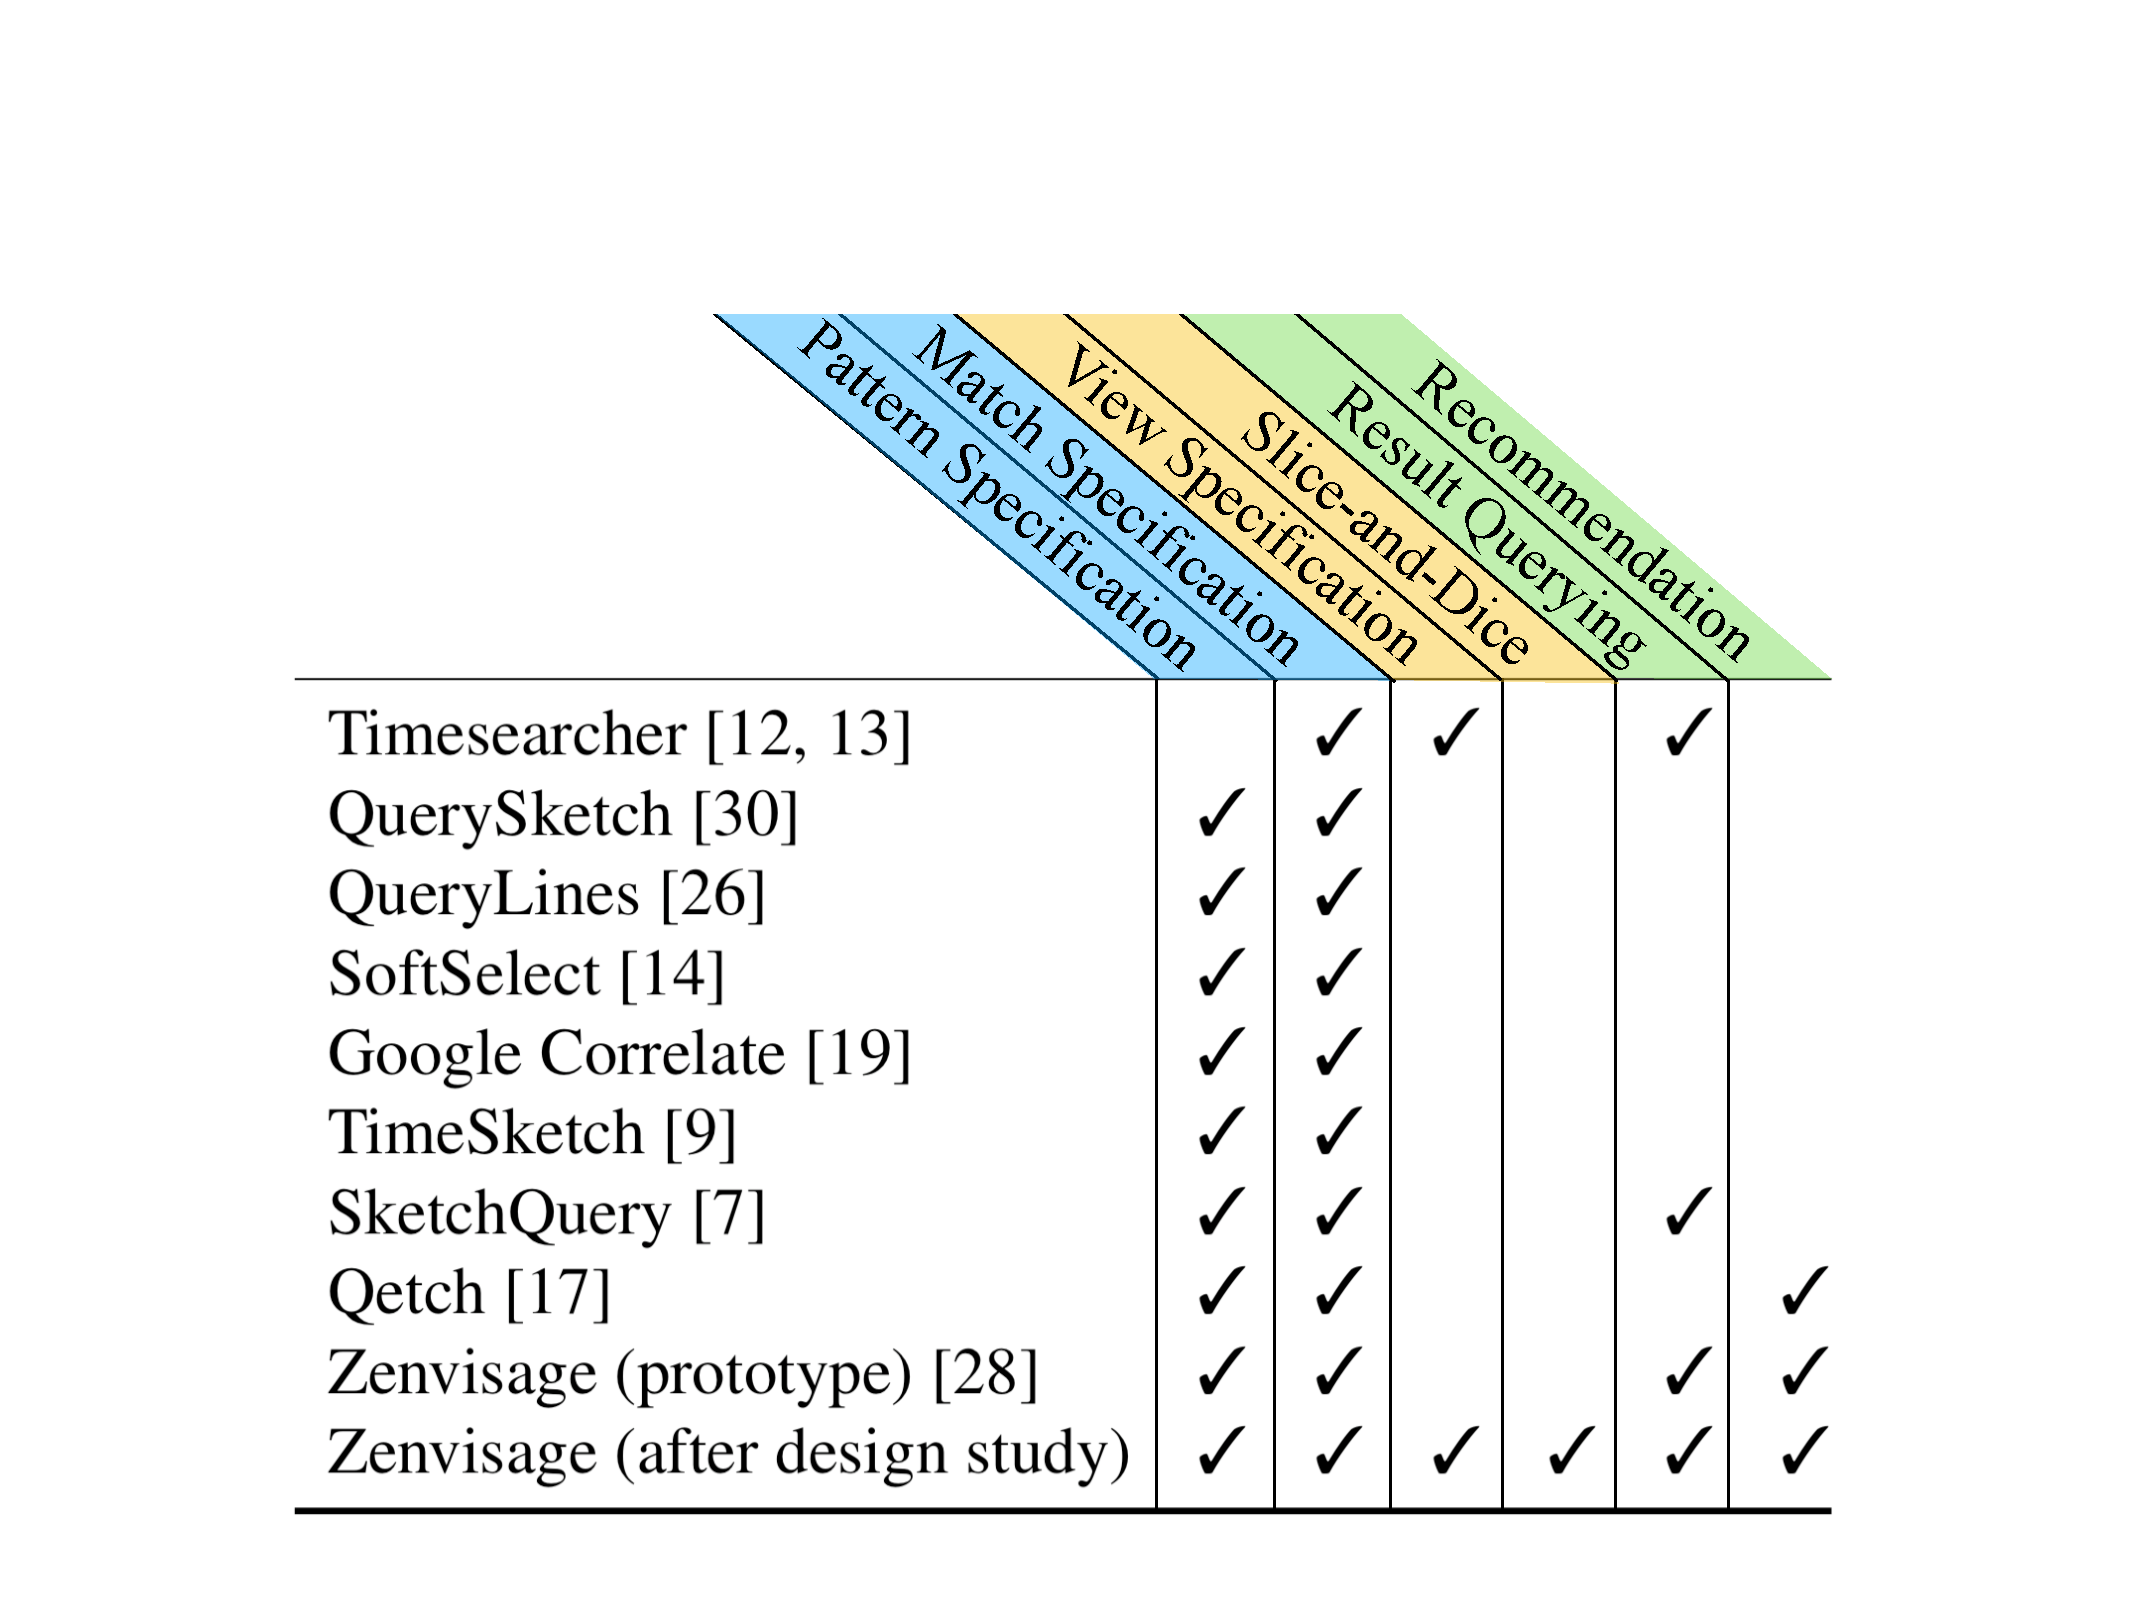
\includegraphics[width=\linewidth]{figures/related_works_table.pdf}
    \caption{Table summarizing the key components of VQSs (columns) covered by past systems (row). Green/red cell color indicates whether this feature exist in the system or not. Column header colors blue, orange, green represents processes: top-down querying, search with context, and bottom-up querying respectively, detailed in Section~\ref{sec:pd_findings}.}
    \label{table:relatedwork}
    \vspace{-27pt}
\end{table}
